\chapter{Background}
This section presents the 
this is short and needs a lot more detail and also figures.

This section briefly reviews the current techniques for lung perfusion and hemodynamic
monitoring, and provides a general overview 
of the state of 3D EIT as used for thoracic imaging and monitoring.


\section{Impedance Imaging}
\label{sec:impedance_imaging}
Impedance imaging has been in use since the early 1900s for geophisical applications.  
Originally introduced as a technique to image below the earth’s surface, 
current was transmitted between two electrodes placed into the ground and any 
anomalies in subsurface conductivity produced deviation 
in the equipotential lines. 
Including current injections and measurements from multiple locations and using known 
electrical properties of geological structures Conrad Schlumberger identified
features of underground geological structures~\parencite{allaud_schlumberger_1977}.

These same techniques can be applied in biomedical applications where
voltage is measured on an array of body surface electrodes 
while current is applied between select electrode pairs (\fref{fig:cur_equip_line}). 
Due to impedance differences associated with biological tissues and their physiological 
function~\parencite{Geddes1967,McAdams1995},
EIT has been proposed for a wide range of applications from thoracic monitoring to neuronal and 
brain imaging~\parencite{Holder1992,Frerichs2016}. 

\begin{figure}
    \centering
   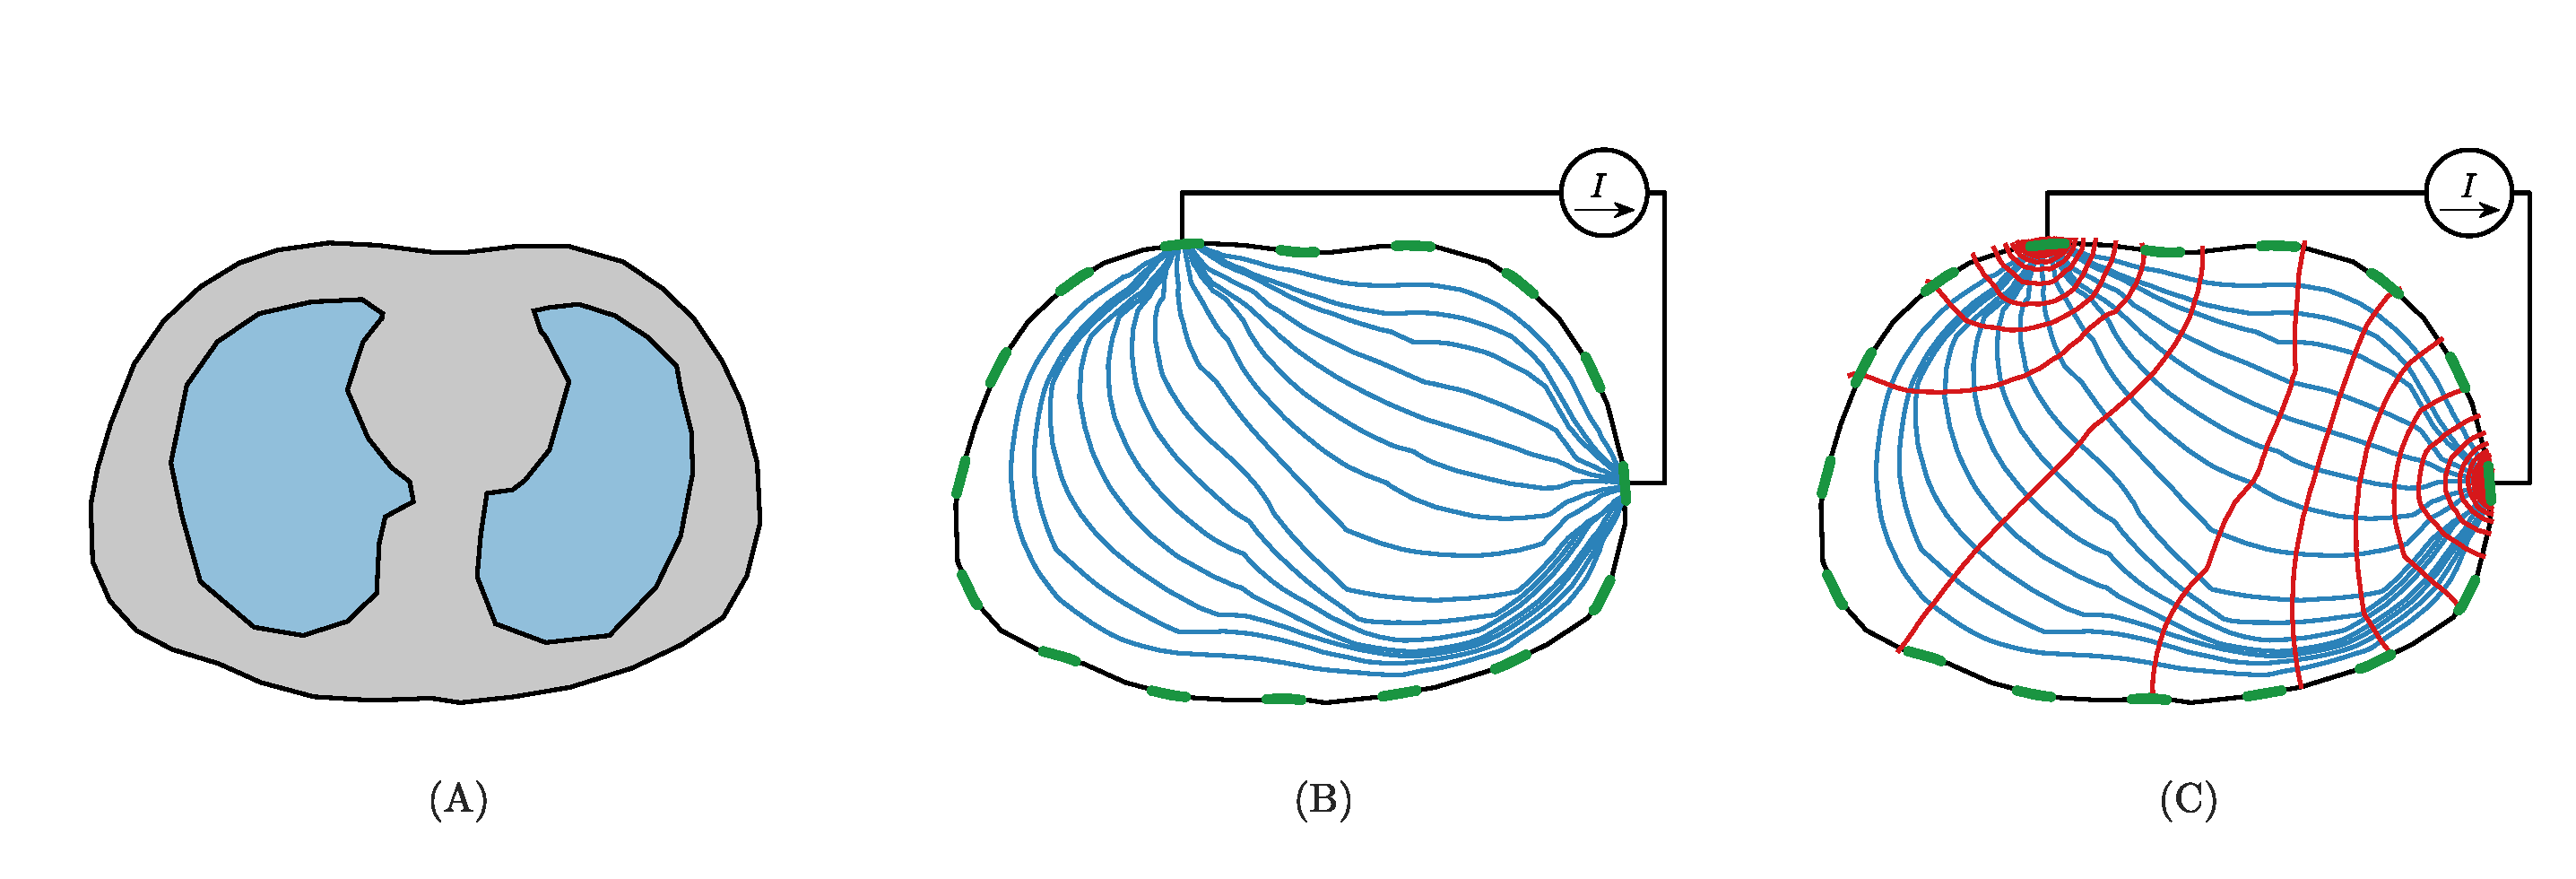
\includegraphics[width=\textwidth]{chapter2-background/imgs/current_and_equipotential_lines.pdf}
   \caption[Current and Equipotential lines]{\label{fig:cur_equip_line} 
   (A) A body comprising tissues of different conductivity, (B) Electrodes are placed on the surface 
   and current is injected between a pair or electrodes. The current pathways are indicated 
   by the blue lines. (C) The resulting equipotential lines within the body.}
\end{figure}

\section{Bioimpedance}
\label{sec:bioimpedance}
In thoracic imaging the most commonly measured 
impedance changes occur due to movement 
of air in the lungs, the flow of blood, and the motion of 
organs~\parencite{adler_electrical_2017}. 
During inhalation, the volume of air in the lungs increases, lowering the 
conductivity of the lung tissue. 
The resistivity of lung tissue varies significantly
between expiration and inspiration giving a value of 7 $\Omega$ m during expiration
and 23 $\Omega$ m during inspiration at 100 kHz~\parencite{witsoe_electrical_1967},
resulting in a
measureable variation in impednace during respiration~\parencite{eyuboglu_vivo_1989}. 
There are also other 
signifant sources of impedance change that make EIT signal intrepretation 
challenging. Simulations have attributed up to 20
percent of the respiratory signal to the effect of 
chest expansion and movement of the chest 
wall~\parencite{adler_impedance_1994}.

The source of impedance changes due to the flow of blood is even more complex. 
Since the resistivity of blood is so much lower than other tissues 
(1.5 $\Omega$ m), the increase of blood due to pulsatile 
flow should decrease the impecance of structures it passes through 
by a detectable amount~\parencite{eyuboglu_vivo_1989}.
It is often assumed that the component of EIT images at the cardiac 
frequency is related to the perfusion of blood, but the exact source of
cardiosynchronus EIT signals is 
unclear~\parencite{patterson_impedance_2010,nguyen_review_2012}.
A continuous flow of blood alone is insufficient 
to induce a significant impednce change, 
as the volume and concentration of the conductive medium is unchanged. 
Any impedance-based measure of perfusion relies on the cardiosynchronous 
EIT signals which have numerous possible sources~\parencite{adler_origins_2017}. 

\subsection{The Cardiac Cycle}
%The following subsection is a brief overview on elements of 
%the cardiac cycle that
%relate to perfusion imaging with EIT.
The cardiac cycle consists of the activity in the heart between the
beginning of one heart beat, and the next. There are two main stages 
of the cardiac cycle: the diastole, when the heart relaxes and is filled 
with blood, and the systole, when contraction of the heart pumps blood to
lungs and all other body systems~\parencite{pappano_cardiovascular_2019}. 
A simplified anatomy of the heart is 
presented in \fref{fig:anatomical_heart}. 
Since ECG recordings are frequently used to synchronize 
EIT data, it is helpful to look at the timing of the cardiac cycle as it 
relates to features of ECG traces. An example ECG waveform is pictured in 
\fref{fig:cardiac_bioimpedance}. 

\begin{figure}
    \centering
    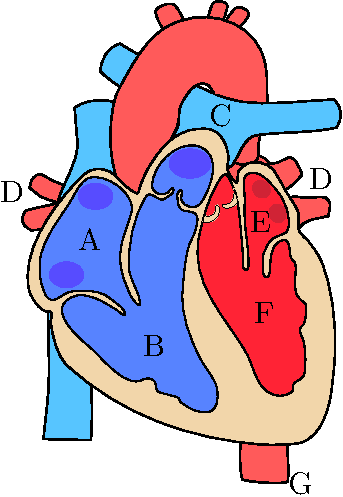
\includegraphics[width=0.6\textwidth]{chapter2-background/imgs/heart_drawing.pdf}
    \caption[Sketch of the anatomical heart]{ The pathway of the blood
    from entry to the heart to the descending aorta is indicated by the
    letters. Deoxygenated blood enters the heart through the right atrium
    (A) where it is moved to the right ventricle (B). From there it passes through 
    the pulmonary artery (C) into the lungs where it perfuses and is oxygenated. 
    Blood return from the lungs through the pulmonary veins (D) then enters 
    the left atrium (E). Finally, the blood is pumped from the left
    ventricle (F) to the rest of the body through the aorta, and the
    descending aorta (G).}
    \label{fig:anatomical_heart}
\end{figure}

During the first stage of the cardiac cycle is the ventricular
diastole, indicated by the P wave on an ECG trace, during 
which the heart relaxes and expands
pulling blood into the ventricles from the 
atria~\parencite{pappano_cardiovascular_2019}. Blood enters the atrium 
on the right side of the heart through the
superior and inferior vena cava and on the left side of the heart, the atrium is 
filled by oxygenated blood from the lungs through the pulmonary 
veins~\parencite{pappano_cardiovascular_2019}.
Next is the atrial contraction during which time the atria pump additional
blood into the ventricles, and the ventricular volume and pressure 
is maximized. At the peak of the ventricular volume, the ventricles contract 
and depolarize which corresponds to the QRS complex~\parencite{pollock_physiology_2021}. 
On the right side of the heart, deoxygenated blood is pumped 
to the lungs where it perfuses into the lung tissue, and on the left side of 
the heart oxygenated blood is pumped to the rest of the body through the 
aorta~\parencite{pappano_cardiovascular_2019}. The smallest volume in the ventricles occurs after 
the ventricular repolarization represented in the ECG by
T wave~\parencite{pollock_physiology_2021}.

\begin{figure}
\centering
\begin{tikzpicture}[line join=round, x=2pt, y=-2pt]
    \tikzset{
        normal ecg/.pic={
            \draw (0,455.0021) -- (11.8345,455.0021);
            \draw (11.8345,455.0021) .. controls (14.2834,454.8958) and
                (14.1385,448.7114) .. (18.8842,448.7114) .. controls (24.2116,448.7114) and
                (23.9695,454.8958) .. (26.3035,455.0021) node[above, xshift=-22pt, yshift=21pt] {P};
            \draw (26.3035,455.0021) -- (40.7723,455.0021) node[below, xshift=5pt, yshift=-25pt] {Q} ;
            \draw (40.7723,455.0021) -- (42.7455,463.0645) -- (46.0339,413.3461) node[above, xshift=0pt, yshift=0pt] {R}
                -- (48.6647,466.4235) -- (51.2955,455.0021) node[below, xshift=-7pt, yshift=-35pt ] {S} ;
            \draw (51.2955,455.0021) -- (61.1605,455.0021);
            \draw (61.1605,455.0021) .. controls (64.4487,454.3298) and
                (65.7118,441.6860) .. (70.3679,441.5241) .. controls (75.2428,441.3542) and
                (76.9447,454.3301) .. (80.2329,455.0021) node[above, xshift=-29pt, yshift=39pt] {T};
            \draw  (80.2329,455.0021) .. controls (81.4852,455.0021) and
                (82.2677,452.8462) .. (84.1792,452.9863) .. controls (85.8717,453.1101) and
                (86.4830,455.0021) .. (87.4678,455.0021); % node[above, xshift=-10pt, yshift=5pt] {U};
            \draw (87.4678,455.0021) -- (100,455.0021);
        }
    }
    \foreach \x in {0}{
    \pic [very thick, scale=1.5] at (\x*50, 0) {normal ecg};
    }
\end{tikzpicture}
\caption[Example ECG waveform]{ An example ECG waveform to compare electrical signals in the 
heart to blood volume changes.
The P wave represents the beginning of the cardiac cycle with the ventricles begin to fill. The QRS complex
corresponds with ventricular depolarization 
and occurs as the ventricles contract they contract.  The beginning of the QRS complex corresponds with 
the maximum ventricular volume. The minimum 
volume in the ventricles occurs after ventricular repolarization represented by the T wave.}
\label{fig:cardiac_bioimpedance}
\end{figure}

\subsection{Bioimpedance of Perfusion}
There are several factors that may contribute some part of 
the impedance change during the cardiac cycle. 
Some of these factors include:
\begin{itemize}
    \item Changes in blood volume within the heart as blood is pumped. As the ventricles 
          fill with blood
          the volume increases and results in a more conductive
          heart~\parencite{nyboer_impedance_1970}.
    \item Variations in arterial and blood vessel volume. Due to the elasticity of arteries 
          and
          blood vessels, the pulsatile flow of blood passing through results in variation of 
          vessel diameter, affecting the impedance~\parencite{eyuboglu_localisation_1987}.
    \item Physical deformation of structures due to motion of the heart. The
          motion of the heart can have significant contribution 
          to cardiosynchronous EIT 
          images~\parencite{proenca_influence_2015,adler_origins_2017}, 
          with simulations showing that heart motion was the 
          main contributor to impedance change due to the 
          ventricle~\parencite{proenca_influence_2015}. 
    \item The orientation of red blood cells. During pulsatile flow the orientation of
          red blood cells changes, which had been shown to affect the impedance of the 
          blood~\parencite{gaw_effect_2010}. 
    \item Ballistic forces in the body generated by the heart. During each
          heartbeat blood is pumped downwards through the descending
          aorta with a large force pushing the rest of the body 
          upwards~\parencite{gordon_certain_1877}. Different directions 
          of flow in the aorta result in a repeating ballistic 
          signal on the rest of the body~\parencite{kim_ballistocardiogram_2016}. This results in 
          motion on the electrodes and body which can introduce significant
          artefacts in EIT signals~\parencite{adler_impedance_1994}.
\end{itemize}

The contribution of each of these factors will ultimately depend on the placement
of the electrodes and the specific geometry and physiology of a patient. 
When imaging changes in stroke volume, changes 
relating to posture, breathing and changes in belt 
position resulted in  changes that overpowers the 
perfusion signals~\parencite{patterson_variability_2001}.  

Despite the challenges of isolating cardiosynchronous EIT signals related to 
perfusion there is still a great interest in 
improving accuracy and stability due to the unique 
advantages offered by EIT over current state-of-the-art methods.

\section{Perfusion Imaging}


\TODO{Discuss the reason for perfusion imaging here}
There is great interest in monitoring and imaging perfusion in the thorax.
Measures and images describing perfusion in the cardiovascular 
system is widely used to diagnose diseases such as pulmonary edema. 
There are several current techniques to image this
\TODO{What methods should be discussed here? Initially thinking 
strictly perfusion and discuss ability to image flow?}


Additional informaion on the function of the cardiovascular system can
improve diagnostic accuracy 

Several techniques are used to monitor and image perfusion in the heart 
and lungs.

There are three main  
and are presented in the following section. 
\TODO{Additional places for inforation for more indepth stuff?}

\subsection{Perfusion Imaging Techniques}
\subsubsection{Microspheres}
\subsubsection{Nuclear medicine}
\subsubsection{MRI}
\subsubsection{CT}
\subsubsection{Thermal diffusion}
\subsubsection{contrast agent}
\subsubsection{Ultrasound}
\subsection{Electrical Impedance Tomography for Perfusion Monitoring}

\section{Electrical Impedance Tomography}
As described in \fref{sec:impedance_imaging} 

\subsection{Imaging Techniques}
There are several challenges with EIT that make absolute EIT imaging difficult. 
The subtle difference in tissue impedance are small relative to artefact introduced 
by unknown boundary locations and electrode 
positions~\parencite{adler_why_2015,adler_electrical_2017,nissinen_compensation_2009}. 
EIT measurements are typically used by 
reconstructing impedance differences between to time points.
Time difference EIT uses a reference frame to image the change in conductivity between 
two points in time and allows for imaging of functional activity such as the inflation of the lungs 
and the flow of blood.
Time-difference EIT is also much more stable in the presence of errors that remain 
constant~\parencite{brown_electrical_2003,adler_electrical_2017}.
Frequency difference EIT is also possible based on the different impedance response 
of tissue types to changing frequencies. Frequency difference uses 
two or more different frequencies and calculates an image based on the change in electrical properties.
Most frequencies used to differentiate between different tissue types are at high frequencies 
where current starts to flow across the cell membranes. 
These high frequencies are out of the range of most current EIT systems and 
frequency changes due to different lower frequencies are limited~\parencite{adler_electrical_2017}.
This thesis uses time-difference EIT to images changes in movemnt and fluid volumes in teh thorax.

\subsection{EIT measurements}
EIT measurements are made on a number of external electrodes placed on the body sorface around
a region of interest. In this thesis we focus on measurements of the thorax. The main aspects
affecting EIT measurements are the electrodes places on the body surface and technical details 
of the current and voltage that are required. 
\subsubsection{Electrodes} \label{sec:electrodes}
EIT is possible using \TODO{How mmuch here? If any? polarizing vs
non polarizing? brief overview of CEM?}
\TODO{electrode impedance on injection vs non-injection measurements}
\TODO{Discuss how and why measurement on injecting electrodes are typically discarded also
talk about this in electrode seciton}

\subsubsection{Current injection and voltage measurement}
To calculate impedance three main conisderations must be made with regard to the 
injected current: the frequency, amplitude and pattern. 

Low frequency currents will 
prefferentially pass around cells through the extracellular
fluid due to the high capacitive componenet of the cell 
membrane~\parencite{foster_whole-body_1996}, wheras high frequency currents will be 
more affected by the capacitive 
componenet~\parencite{holder_electrical_2004}. 
Since EIT requires a linear relationship between the measured voltages and 
tissue impedance to produce valid reconstructions,
it is important to select frequencies of less than 1 MHz to ensure that cell 
and neural membrane is not the dominant factor in the impedance 
measurements~\parencite{barber_applied_1984}.
Impedance measurements below 100 KHz have shown to be primarily rsitive on lung
tissue~\parencite{witsoe_electrical_1967}, and most EIT systems use
frequencies between 10 kHz and 1 Mhz~\parencite{holder_electrical_2004}.

The selection of current amplitudes is selected based on the \TODO{Ask Andy}.

The pattern of current injection and voltage measurement is commonly refered to in EIT 
as the stimulation and measuremnt pattern. Typically a current is injected between two electrodes
while the resulting voltages are measured between asjacent pairs. The two most common injection 
patterns are adjacent, and ``skip 4''. Examples of these measurement patterns are shown in 
\fref{fig:stim_meas_bkgnd} on a 16 electrode system. The terms adjacent and skip 4 describe 
the space between pairs of injecting or measurement electrodes. 
Regardless of the pattern, a frame of EIT data is generated in the same way. 
Current is injected between a pair of electrodes as voltage is measured between all 
remaining pairs, then current is injected between the next pair of electrodes and
voltages are measured again. This results in voltage measurements on each electrode 
pair for every current injection. For a 16 electrode system this results in 
256 measurements in each frame. For a 32 electrode system there are 1024. As mentioned in 
\fref{sec:electrodes}, voltage measurements made on the stimulating electrodes
are often removed resulting in 208 measurements per frame on a 16
electrode system, and 928 measurements per frame on a 32 electrode system.  

\begin{figure}
    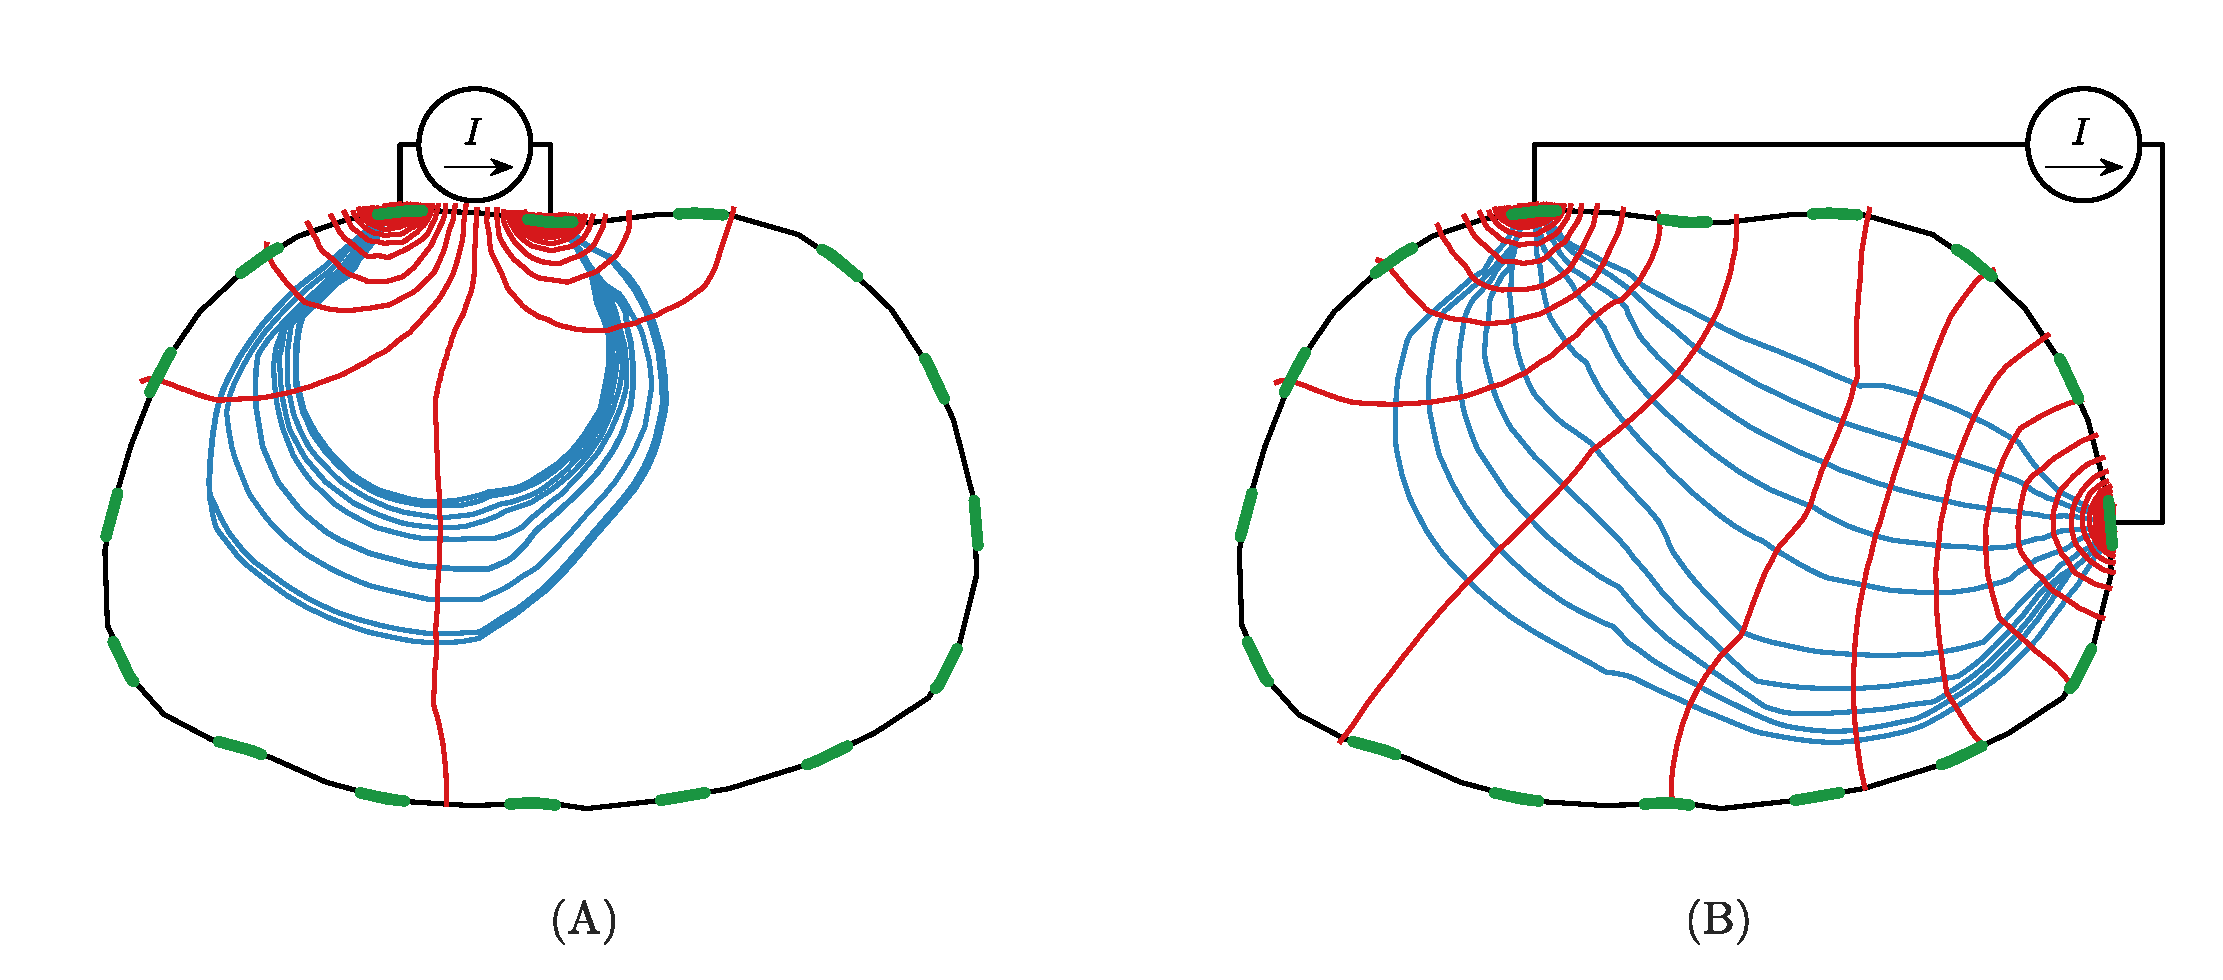
\includegraphics[width=\textwidth]{chapter2-background/imgs/common_stim_meas_patterns.pdf}
    \caption[Adjacent and "skip 4" stimulation patterns]{\label{fig:stim_meas_bkgnd} 
    Two common stimulation patterns are simulated on a simple human model showin in 
    \fref{fig:cur_equip_line}. Injected current is shown in blue and the resulting equipotential 
    lines are shown in red.
    (A) An exmaple of an adjacent stimulation pattern. Current is injected between 
    pairs of adjacent electrodes. For each current injection voltage is 
    measured between all sequential pairs. 
    (B) An example of the ``skip 4'' injection pattern. Current is injected between every
    5\textsuperscript{th} electrode skipping 4 between the injecting electrodes. 
    during each current injection, voltage measurements are made using the same skip 4 
    pattern between each of the 16 electrodes and their corresponding pair. 
    A single frame of data is generated by all measurements made for each possible injection
    pattern. For 16 electrodes this results in 256 meaasurements.}
 \end{figure}

\subsection{Image Reconstruction}


\subsection{Forward Problem}
Using the static 
formulations of Maxwell's equations, the potential distribution $u$ can be used 
compute the conductivity $\rho$ and generate images.
We are able to use the static form of Maxwell's equations 
% Derivation and explanation here

\subsection{Discretization and the Finite Element Method}


\subsubsection{2D reconstruction}

\subsubsection{3D Reconstruction}
The majority of EIT measurements are done with a single ring of external electrodes but 
in practice, electrical current cannot  be confined to a single plane
and using a two dimensional electrode configuration can significantly
impact the capabilities of \acrshort{eit}~\parencite{Rabbani1991}.
The use of 3D electrode configurations in \acrshort{eit}
was introduced in 1996~\parencite{Metherall1996} to overcome the 
inherent limitations of 2D measurements, but it is still not widely used today.
It is thought this is due to the increased complexity of 3D images
and the subsequent analysis~\parencite{Grychtol2019}.

It has been shown that externally placed 3D electrode configurations
consisting of two electrode planes
can improve the sensitivity distribution and image quality~\parencite{Grychtol2016},
but there is still limited sensitivity in the central-most regions 
of the chest.
The concept of using internal esophageal electrodes has been presented
previously~\parencite{Pilkington1989,Schuessler1995}
as a method to improve internal sensitivity 
and reconstruction quality,
but has not been widely used or simulated.
Several studies have shown that there may be several advantages to using an internal
electrode in \acrshort{eit} recordings; 
Measurements with an internal electrode have been 
shown to reconstruct images equally as well as configurations with 
twice as many external electrodes~\parencite{Schuessler1995},
and have shown an increase in sensitivity in a central region 
of interest~\parencite{Kwon2013,Czaplik2014,Farooq2014}.

\subsubsection{GREIT}

\subsubsection{Image Regularization}


\subsection{Internal Electrodes}
\subsubsection{Motion Correction} \label{sec:motion_correction}
\subsubsection{Internal Reference Electrodes}
\subsubsection{Inverse Source localization (time permitting)}









% TODO in the thesis go into absolute imaging vs time difference imaging in depth here!!!

\section{Perfusion monitoring}
\subsection{Contrast agent injection}
\subsection{Frequency Filtering}


Monitoring lung ventilation is one of the most
established clinical uses of 
\acrshort{eit}, presented initially by Barber and Brown~\parencite{Barber1984}.
EIT has also been used as a tool to monitor blood 
perfusion~\parencite{Brown1992} and hemodynamic parameters such as 
cardiac output~\parencite{Braun2018} and blood pressure~\parencite{Sola2011,Proenca2017}. 
While the spatial resolution of \acrshort{eit} is much lower than 
intermittent imaging techniques such as \acrfull{ct} or \acrfull{mri},
\acrshort{eit} can have a high temporal resolution enabling continuous or frequent 
monitoring without concerns regarding radiation exposure.
This thesis focuses on time difference EIT for thoracic hemodynamic imaging and monitoring applications. 

EIT is sensitive to the movement of blood in two main ways. First, a conductivity-contrasting 
bolus solution injected into a vein or artery can be used to image the transit of blood through the body
and second, the pulsatile changes in conductivity at the cardiac frequency can be isolated 
through digital filtering~\parencite{Leathard1994}.
This document proposes methods and techniques to identify and isolate these impedance variations
to monitor lung perfusion and 
aortic flow.

A perfusion scan is a technique for imaging the blood flow through the lungs
and when compared with ventilation images can be used to detect pulmonary embolisms
when a mismatch is identified. Clinically pulmonary perfusion is done using 
lung nuclear medical imaging such as \acrfull{spect}~\parencite{Parker2012}. Radio-isotopes are inhaled through a mask 
for ventilation imaging and injected into the blood to image pulmonary perfusion. 
Images taken on a gamma camera are compared to look for a mismatch between the ventilation
and perfusion distribution. This method of 
measuring lung perfusion is slow and exposes the subject to low-dose radiation.

EIT has been evaluated for its ability to measure cardiac output and
lung perfusion since the late 1980s~\parencite{Eyuboglu1989,Blottt1992,Brown1992,Frerichs2002}. 
Since then, various configurations of EIT have been evaluated~\parencite{Borges2012,Nguyen2015}.
Due to the speed and safety of measurement acquisition, EIT might be used to continuously monitor 
perfusion in subjects.

There are two main challenges with perfusion monitoring using EIT. First, impedance change due to ventilation 
is 10 times larger than the impedance change due to cardiac-frequency pulsatile activity~\parencite{Deibele2008}
and second, the pulsatile activity outside the lung region can overwhelm the lung perfusion signal~\parencite{Stowe2019}. 
There are several techniques available to mitigate the difference 
in magnitude such as: pausing ventilation; administering a 
conductivity-contrasting bolus through the heart and lungs via the jugular~\parencite{Frerichs2002};
and digital filtering to isolate activity at the cardiac frequency~\parencite{Leathard1994}. 

When breathing is paused, the signals based only on the cardiac activity can be more easily extracted. 
It was found that during apnoea the global impedance recorded with EIT measurements corresponded with stroke volume 
measured using the 
thermodilution method with a pulmonary arterial catheter~\parencite{Fagerberg2009}.
Ventilation perfusion ratios have been calculated during apnoea by comparing 
ventilation and perfusion signal amplitude with a specified region of 
interest~\parencite{Fagerberg2009a}.
There is some concern that the perfusion measured during apnoea may not accurately represent 
true perfusion during regular respiration as the apnoea impacts the regular respiratory cycle~\parencite{Leonhardt2012}.

Using the conductivity-contrasting bolus injection EIT perfusion imaging has been compared to 
SPECT measurements, and blood flow has been imaged from the right heart into the lungs and back into the left heart
using 5-10\% hypertonic saline~\parencite{Frerichs2002,Borges2012}. This technique is promising 
for imaging lung perfusion, but is slow and requires the placement of a venous catheter 
and repeated saline injections to obtain perfusion measures. 

The final method to calculate perfusion using EIT is through filtering to isolate the 
cardiac related signal. Previous work has shown that principal component analysis (PCA) 
can be used to separate ventilation and cardiac frequency signals and identify the component 
related to the heart~\parencite{Deibele2008}. Once the cardiac-frequency component of the 
EIT signal is identified the pulmonary component must also be isolated. Other than visual 
identification of the lung region or manually selecting a region of interest,
there are few good solutions for isolating pulsatile activity within the lung region.

The use of 3D configurations to differentiation between pulsatile activity 
in the heart and lungs could allow for an improved perfusion measure 
using EIT, and a means of continuously monitoring perfusion during ventilation.

%\section{Aortic flow monitoring}
%
%Continuous bedside monitoring appears to be one of the most
%promising future applications of \acrshort{eit} due to the high 
%temporal resolution, and concerns with other imaging modalities 
%and the associated radiation 
%exposure. 
%
%%There are several hemodynamic parameters that are widely used to asses cardiovascular 
%%health. One of the most used is cardiac output (CO), the amount of blood pumped through the
%%heart in one minute.
%%The two most used method is
%%thermodilution using a Swan-Ganz catheter~\parencite{Khalil1963} in the pulmonary artery, 
%%which determines CO by injecting a solution with a known temperature and 
%%measuring the temperature change~\parencite{ReuterDaniel2010}. This method is considered the gold standard of 
%%CO monitoring~\parencite{Joosten2017}.
%
%Another potential use of EIT is to replace invasive monitoring techniques
%such as catheterized measurements of pulmonary arterial pressure.
%Recent studies have evaluated EIT as a method of determining 
%pulmonary arterial pressure using pulse wave velocity in the 
%descending aorta in 2D~\parencite{Braun2018a,Proenca2017,Proenca2016}.
%EIT was a used in conjunction with ECG signals and shown to have a high correlation
%with pulmonary arterial pressure values from from Doppler echocardiography~\parencite{Proenca2016}.
%
%An analysis of hemodynamic measures using EIT found that measures of stroke 
%volume and pulmonary arterial pressure are sensitive to electrode placement and
%interference from pulmonary signals~\parencite{Braun2018a}. 
%The solution proposed in this document uses an arrangement of internal electrodes placed in the 
%esophagus adjacent to the aorta to increase the sensitivity to changes and improve detection 
%accuracy and elimination of pulmonary signals.
%
%Improving tracking and imaging of the aorta is also important because it
%has additional clinical uses: it  can be used as a physiological landmark to identify
%the back of the lungs, and can be used to continuously monitor blood pressure by
%calculating the pulse transit time. 



\acrshort{eit} has been used clinically to monitor lung perfusion 
in an animal model~\parencite{Leonhardt2012,Nguyen2012}, and it is theorized that 
the use of an internal electrode for increased sensitivity may allow for 
imaging of blood flow in the aorta. 
There is great interest in monitoring cardiac parameters
using \acrshort{eit} to determine \acrfull{sv}~\parencite{Proenca2017,Braun2018}, and increased
sensitivity close to the heart also has the potential to improve
these measures.

While there have been some studies researching electrode placement for cardiac
imaging in 2D~\parencite{Noordegraaf1996} and 
3D electrode configurations~\parencite{Graham2007}, there has 
been little research into determining the optimal 3D external electrode configurations
for imaging the heart and aorta. 

Additionally when using alternate electrode configurations the current injection and 
measurement patterns must also be investigated. It has been suggested that  an internal electrode
in 2D
should not be used for current injection in asymmetrical models
as the reconstruction performance deteriorates~\parencite{NasehiTehrani2012}. 
It is unclear 
to what degree injection patterns affect the resulting sensitivity when
internal electrodes and alternate electrode arrangements are used in 3D.

This work aims to investigate internal and 
external electrode configurations for use in imaging blood movement 
in the thorax, and develop techniques to extract measures of 
aortic flow and lung perfusion from these reconstructions.

%\subsubsection{3D \acrshort{eit} image reconstruction}
%It has been shown that when the continuous boundary voltages of a surface are
%known, there is a unique solution to the inverse problem used to calculate internal 
%conductivity~\parencite{Calderon2006},
%but EIT uses discrete measurements of boundary voltage 
%and there is no unique solution. 
%
%In order to reconstruct EIT images prior information and smoothing 
%must be used to obtain a solution. There are several reconstruction methods used in 
%EIT including Tikhonov regularization~\parencite{Tikhonov1977} and 
%standardized methods for EIT such as GREIT~\parencite{Adler2009}.
%A version of GREIT for 3D reconstructions~\parencite{Grychtol2016}
%is used in this work.
